\documentclass[11pt,a4paper]{article}

\usepackage[utf8]{inputenc}
\usepackage[T1]{fontenc}
\usepackage[spanish]{babel}
\usepackage{amsmath,amssymb}
\usepackage{graphicx}
\usepackage{booktabs}
\usepackage{listings}
\usepackage[margin=2.5cm]{geometry}
\usepackage{array}
\usepackage{tikz}
\usetikzlibrary{babel}

\lstset{
  basicstyle=\ttfamily\small,
  breaklines=true,
  frame=single,
  language=Python
}

\title{Taller semana 12: FFT y Sistemas de Modulación}
\author{CE1110: Análisis de Señales Mixtas \\ Integrantes: Jorge Pablo Porras \\ Marcelo Matey Rodriguez
\\ Josue Adrian Perez Perez}
\date{30 de octubre de 2026}

\begin{document}
\maketitle

% =====================================================================
% PARTE 1: prototipado de frecuencias del sistema (llenar) 
% =====================================================================
\section{Parte 1: Frecuencias del sistema}
\subsection{Objetivo}
Prototipar en Python el sistema completo de tres nodos tal como operará en
los microcontroladores, para definir y verificar las frecuencias de trabajo
antes de implementarlo en hardware. A diferencia de la Tarea~1, donde cada
método procesó el archivo completo de una sola vez, la simulación reproduce
las restricciones del sistema embebido: la señal se procesa por bloques a
medida que llega, cada nodo conserva su propio estado entre bloques, el ADC
cuantiza a 12~bits y los nodos se comunican mediante tramas de bytes con
detección de errores.
 
\subsection{Arquitectura simulada}
La Figura~\ref{fig:arquitectura} muestra el flujo de datos. Cada nodo se
modela como un objeto cuyo estado interno es lo que recuerda entre bloques,
y cada iteración del ciclo principal representa la llegada de un bloque de
512 muestras nuevas, es decir, $512/f_s = 32$~ms de tiempo real.
 
\begin{figure}[h]
  \centering
  \begin{tikzpicture}[
      nodo/.style={draw, rounded corners, align=center, minimum height=1.1cm,
                   minimum width=2.6cm, font=\small},
      flecha/.style={->, >=stealth, thick},
      etiqueta/.style={font=\scriptsize, align=center}]
    \node[nodo] (fuente) at (0,0) {Señal útil\\+ interferencia};
    \node[nodo] (n1) at (4,0) {Nodo 1\\ADC + FFT\\+ estimación};
    \node[nodo] (n2) at (9,1.5) {Nodo 2\\Notch IIR\\adaptativo};
    \node[nodo] (n3) at (9,-1.5) {Nodo 3\\FFT/IFFT\\+ métricas};
    \draw[flecha] (fuente) -- (n1);
    \draw[flecha] (n1) -- node[etiqueta, above left] {trama 1034 B} (n2);
    \draw[flecha] (n1) -- node[etiqueta, below left] {trama 1034 B} (n3);
    \draw[flecha] (n2) -- node[etiqueta, right] {salida\\temporal} (n3);
  \end{tikzpicture}
  \caption{Arquitectura simulada. Cada trama transporta 512 muestras en
  \texttt{int16} y la frecuencia de interferencia estimada por el Nodo~1.}
  \label{fig:arquitectura}
\end{figure}
 
\begin{itemize}
  \item \textbf{Nodo 1} quita el nivel de DC, forma una ventana de $N=1024$
        muestras (bloque anterior y bloque nuevo), aplica la ventana de Hann,
        calcula la FFT y estima la frecuencia de la interferencia como el
        pico más alto por encima de la banda útil. Si el pico no sobresale al
        menos 20~dB sobre la mediana del espectro, se considera que no hay
        interferencia tonal y envía frecuencia~0.
  \item \textbf{Nodo 2} diseña un notch IIR de segundo orden en la frecuencia
        recibida y filtra el bloque conservando el estado del filtro entre
        bloques. Solo recalcula los coeficientes si la frecuencia cambia más
        de 0.5~Hz, y deja pasar la señal si recibe frecuencia~0.
  \item \textbf{Nodo 3} aplica el método espectral de la Tarea~1 (ganancia de
        Wiener y notch espectral) por bloques, reconstruyendo la salida por
        \emph{overlap-add}.
  \item Un \textbf{oráculo} externo, que sí conoce la señal limpia, calcula
        las métricas de ambos métodos; en el sistema real esa referencia no
        está disponible.
\end{itemize}
 
Cada trama contiene sincronía (2~B), número de bloque (2~B), frecuencia
estimada (2~B, en unidades de $1/8$~Hz), prominencia del pico (2~B), las
512 muestras (1024~B) y un CRC-16 (2~B), para un total de 1034~B. El código
está en \texttt{src/simulacion\_sistema.py}.
 
\subsection{Frecuencias del sistema y criterios de diseño}
 
\begin{table}[h]
  \centering
  \small
  \begin{tabular}{>{\raggedright\arraybackslash}p{3.8cm}>{\raggedright\arraybackslash}p{3.4cm}>{\raggedright\arraybackslash}p{7.4cm}}
    \toprule
    Parámetro & Valor & Criterio \\
    \midrule
    Muestreo nominal $f_s$ & 16\,000~Hz & Nyquist en 8\,kHz, por encima de toda
      componente útil o interferente; coincide con las señales de prueba. \\
    Muestreo real medido & $\approx 16\,220$~Hz & Medido en la Pico (Parte~2);
      el temporizador no da exactamente $f_s$. \\
    Tamaño de FFT $N$ & 1024 muestras & Potencia de 2 (requisito de la FFT de
      \texttt{ulab}); ventana de 64~ms. \\
    Salto entre bloques & 512 muestras & Solapamiento de 50\,\%; un bloque nuevo
      cada 32~ms (límite de tiempo real). \\
    Resolución $\Delta f = f_s/N$ & 15.6~Hz & Separa la interferencia de los
      tonos útiles. \\
    Banda útil & 300--1500~Hz & Contiene los tonos de la Parte~2. \\
    Tonos útiles & 440, 880, 1320~Hz & Los mismos del emisor (Parte~2). \\
    Interferencias & 1750 y 2500~Hz & Fuera de la banda útil y a más de
      400~Hz del tono útil más cercano; dos valores para probar la
      adaptación. \\
    Ancho del notch ($Q=10$) & 175~Hz en 1750~Hz; 250~Hz en 2500~Hz & $f_0/Q$; no
      alcanza a los tonos útiles. \\
    Filtro antialiasing & corte bajo 8\,kHz & Evita que componentes sobre
      $f_s/2$ se reflejen en la banda útil. \\
    Portadora PWM (propuesta) & $\approx 30.5$~kHz & $125~\text{MHz}/4096$ con
      12~bits; muy por encima de la banda de audio para filtrarla. \\
    UART & 460\,800~baudios & Una trama tarda 22.4~ms ($< 32$~ms);
      115\,200~baudios no alcanza (89.8~ms). \\
    \bottomrule
  \end{tabular}
  \caption{Frecuencias y parámetros prototipados.}
  \label{tab:frecuencias}
\end{table}
 
\paragraph{Frecuencia aparente.}
Como la Pico muestrea a $\approx 16\,220$~Hz pero los nodos suponen
$16\,000$~Hz, un tono de $f$~Hz se observa en la frecuencia aparente
$f \cdot 16\,000/16\,220$; por ejemplo, la interferencia de 1750~Hz se ve en
1726.3~Hz. Esto no afecta al filtrado, porque el Nodo~1 estima y el Nodo~2
diseña el notch con la misma $f_s$: lo que importa es la frecuencia
normalizada (ciclos por muestra), que es idéntica para ambos. La simulación
genera la señal a 16\,220~Hz para reproducir esta condición real.
 
\paragraph{Interpolación parabólica.}
Con $\Delta f = 15.6$~Hz, tomar el bin del máximo produce errores de hasta
$\Delta f/2 \approx 7.8$~Hz, y con ese error el notch atenúa la interferencia
solo unos 21~dB. Por eso el Nodo~1 ajusta una parábola a $\ln|X[k]|$ en el
máximo $k$ y sus dos vecinos:
\begin{equation}
  p = \frac{1}{2}\,\frac{\alpha - \gamma}{\alpha - 2\beta + \gamma}, \qquad
  \hat f = (k + p)\,\frac{f_s}{N},
\end{equation}
con $\alpha, \beta, \gamma = \ln|X[k-1]|, \ln|X[k]|, \ln|X[k+1]|$.
 
\subsection{Validación de la simulación}
Cada nodo se verificó contra una referencia independiente
(Tabla~\ref{tab:validacion}). La equivalencia exacta del Nodo~2 y la
reconstrucción con ganancia unitaria del Nodo~3 demuestran que el estado se
conserva correctamente entre bloques. La diferencia inicial del Nodo~3
respecto a la Tarea~1 se debe a que, en tiempo real, la estimación de ruido
no puede inicializarse con muestras futuras; decae unas diez veces por
segundo porque la estimación se promedia con factor 0.9 por bloque.
 
\begin{table}[h]
  \centering
  \small
  \begin{tabular}{>{\raggedright\arraybackslash}p{1.4cm}>{\raggedright\arraybackslash}p{9.2cm}>{\raggedright\arraybackslash}p{3.8cm}}
    \toprule
    Nodo & Prueba & Resultado \\
    \midrule
    1 & Error de estimación de 1750~Hz, con / sin interpolación & 0.048 / 7.51~Hz \\
    1 & Error de estimación de 2500~Hz, con / sin interpolación & 0.193 / 2.66~Hz \\
    1 & Falsas detecciones con solo tonos útiles o ruido blanco (50 bloques) & 0 \\
    2 & Coeficientes propios vs.\ \texttt{scipy.signal.iirnotch} & $2.2\times10^{-16}$ \\
    2 & Filtrado por bloques vs.\ señal completa & 0 (idéntico) \\
    3 & Reconstrucción con ganancia unitaria & $5.6\times10^{-16}$ \\
    3 & Diferencia vs.\ Tarea~1 en el 1.\textsuperscript{er} / 6.\textsuperscript{o} segundo & $2\times10^{-1}$ / $5\times10^{-8}$ \\
    Tramas & 5\,\% de tramas alteradas en el canal & todas detectadas por CRC \\
    \bottomrule
  \end{tabular}
  \caption{Validación de cada nodo de la simulación.}
  \label{tab:validacion}
\end{table}
 
\subsection{Resultados}
Se usó una señal con los tonos útiles de la Tabla~\ref{tab:param}, SNR de
entrada de 5~dB y una interferencia que salta de 1750 a 2500~Hz en
$t = 3$~s. La Figura~\ref{fig:seguimiento} muestra que el Nodo~1 sigue el
cambio bloque a bloque, y la Tabla~\ref{tab:resultados} resume el desempeño
en régimen estable (sin los dos primeros bloques de cada tramo).
 
\begin{figure}[h]
  \centering
  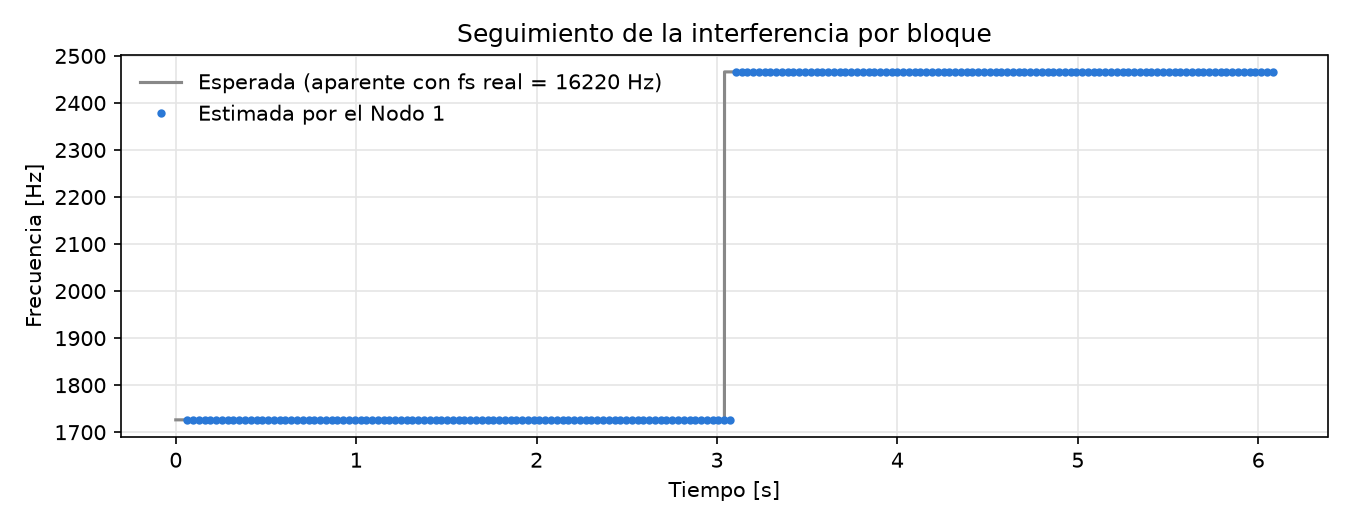
\includegraphics[width=0.9\textwidth]{../resultados/figuras/simulacion_seguimiento_interferencia.png}
  \caption{Frecuencia de interferencia estimada por el Nodo~1 en cada bloque,
  frente a la frecuencia aparente esperada.}
  \label{fig:seguimiento}
\end{figure}
 
\begin{table}[h]
  \centering
  \begin{tabular}{lcc}
    \toprule
    & Temporal (Nodo 2) & Espectral (Nodo 3) \\
    \midrule
    $\Delta$SNR, interferencia en 1750~Hz & +19.5~dB & +34.7~dB \\
    $\Delta$SNR, interferencia en 2500~Hz & +24.7~dB & +39.5~dB \\
    Energía útil conservada & $\geq 99.6$\,\% & $\geq 99.9$\,\% \\
    Latencia de procesamiento & $\approx 0$ & 1 bloque (32~ms) \\
    Latencia de adaptación al salto & 2 bloques (64~ms) & 1 bloque (32~ms) \\
    \bottomrule
  \end{tabular}
  \caption{Desempeño del sistema simulado en régimen estable.}
  \label{tab:resultados}
\end{table}
 
\subsection{Discusión}
Ambos métodos se adaptan al cambio de frecuencia, lo que no era posible con
el notch fijo de la Tarea~1. El método espectral reduce más el ruido, pero
introduce un bloque de latencia: por el \emph{overlap-add}, la salida de un
bloque solo está completa cuando llega el siguiente. El notch entrega cada
muestra de inmediato, pero tarda un bloque más en adaptarse, porque depende
de que el Nodo~1 detecte la nueva frecuencia y se la envíe.
 
El notch rinde 5~dB más con la interferencia en 2500~Hz que en 1750~Hz. La
razón es la distorsión de fase sobre los tonos útiles cercanos: en 1320~Hz
el notch introduce un desfase de $-10.1^\circ$ cuando está en 1750~Hz y de
solo $-4.4^\circ$ cuando está en 2500~Hz. El MSE compara muestra a muestra,
por lo que penaliza ese desfase aunque la amplitud casi no cambie.
 
El tramo de 1750~Hz produjo $\Delta\text{SNR} = 19.5$~dB para el notch, igual
al valor obtenido en la Tarea~1 con el archivo completo (19.45~dB). Que dos
implementaciones distintas coincidan respalda la validez de la simulación.
 
\subsection{Limitaciones}
\begin{itemize}
  \item La simulación no reproduce el tiempo de ejecución. En la Parte~2, el
        análisis de un bloque tomó $\approx 100$~ms en la Pico, por encima de
        los 32~ms disponibles por bloque. Se debe medir por separado el
        tiempo de la FFT de \texttt{ulab} y el de la búsqueda de picos, que en
        el receptor recorre los bins con un ciclo de Python; el Nodo~1 propuesto
        solo necesita el máximo por encima de la banda útil, que puede
        obtenerse con una operación vectorizada.
  \item Se usaron tonos sintéticos sin el trayecto acústico real
        (parlante, sala y micrófono), ni la respuesta en frecuencia de esos
        elementos.
  \item El emisor actual (Parte~2) genera solo los tonos útiles; para probar
        los Nodos~2 y~3 en hardware debe agregarse la interferencia de 1750
        y 2500~Hz.
  \item Los resultados corresponden a una sola corrida por condición.
\end{itemize}
 

% =====================================================================
% PARTE 2: emisor con frecuencias establecidas
% =====================================================================
\section{Parte 2: Emisor con frecuencias establecidas}

\subsection{Objetivo}
Generar una señal de prueba formada por las frecuencias definidas en la
parte~1 y usarla como entrada del receptor implementado en la
Raspberry Pi Pico~W, para comprobar que el receptor identifica cada
componente en frecuencia.

\subsection{Señal generada}
El emisor produce una suma de tres senoidales:
\begin{equation}
  x[n] = \sum_{i=1}^{3} A_i \,\sin\!\left(\frac{2\pi f_i\, n}{f_s} + \varphi_i\right),
  \qquad n = 0,1,\dots,N_{\text{tot}}-1
\end{equation}
con los parámetros de la Tabla~\ref{tab:param}. Después de sumar, la señal
se normaliza para que su valor máximo en magnitud sea $0.6$ de la escala
completa.

\begin{table}[h]
  \centering
  \begin{tabular}{cccc}
    \toprule
    Componente & $f_i$ (Hz) & $A_i$ (relativa) & $\varphi_i$ (grados) \\
    \midrule
    1 & 440  & 1.00 & $0$   \\
    2 & 880  & 0.55 & $35$  \\
    3 & 1320 & 0.30 & $-50$ \\
    \bottomrule
  \end{tabular}
  \caption{Parámetros de las componentes del emisor.}
  \label{tab:param}
\end{table}

\subsection{Criterios de diseño y justificación}

\paragraph{Frecuencia de muestreo.}
Se usa $f_s = 16000$~Hz. Por el teorema de muestreo, la máxima frecuencia
representable es $f_s/2 = 8000$~Hz, mucho mayor que la componente más alta
($1320$~Hz), por lo que no hay aliasing. Además, es del mismo orden que la
frecuencia de muestreo efectiva del receptor ($\approx 16220$~Hz medida en
la Pico), lo que evita trabajar con tasas muy distintas entre emisor y
receptor.

\paragraph{Frecuencias, amplitudes y fases.}
Las tres frecuencias son enteras y relacionadas armónicamente
($440$, $2\cdot 440$, $3\cdot 440$~Hz). Las amplitudes decrecen
($1.00 > 0.55 > 0.30$) para que el receptor tenga que detectar componentes
con niveles distintos y no solo la más fuerte. Las fases distintas de cero
verifican que la detección de picos en la magnitud del espectro no depende
de la fase inicial de cada componente.

\paragraph{Resolución espectral.}
El receptor trabaja con bloques de $N = 1024$ muestras. La resolución en
frecuencia es
\begin{equation}
  \Delta f = \frac{f_s}{N} \approx \frac{16220}{1024} \approx 15.8\ \text{Hz}.
\end{equation}
Las frecuencias del emisor no coinciden exactamente con un bin
(por ejemplo, $440/15.8 \approx 27.8$), por lo que aparece fuga espectral;
el receptor aplica una ventana de Hann para reducirla.

\paragraph{Rampa al inicio y al final.}
Los primeros y últimos $20$~ms ($0.02\cdot 16000 = 320$ muestras) se
multiplican por una rampa $\sin^2$, para evitar un salto brusco
(chasquido) al comenzar y terminar la reproducción, que de otra forma
introduciría energía en todo el espectro.

\paragraph{Formato de salida.}
La señal se guarda como archivo WAV de $16$~bits con signo, a
$f_s = 16000$~Hz y duración de $10$~s, para reproducirla desde la
computadora.

\paragraph{Reproducción desde la computadora.}
Según lo confirmado por el profesor en el canal de Discord del curso
(captura en la Figura~\ref{fig:discord}), el hardware del proyecto es la
Pico y el micrófono, y el audio puede reproducirse desde la computadora.
Por eso el emisor se implementa como un programa en la computadora que
genera el archivo \texttt{tonos.wav}, y el micrófono conectado a la Pico
recibe la señal por el aire.

\begin{figure}[h]
  \centering
  % \includegraphics[width=0.8\textwidth]{discord.png}
  \fbox{\parbox{0.7\textwidth}{\centering Captura de la conversación con el profesor \\ (insertar \texttt{discord.png})}}
  \caption{Confirmación del profesor sobre el hardware y la reproducción de audio desde la computadora.}
  \label{fig:discord}
\end{figure}

\subsection{Implementación}
El emisor está en \texttt{emisor\_tonos.py} (Python con \texttt{numpy} y
\texttt{scipy}). Los pasos son:
\begin{enumerate}
  \item Construir el vector de tiempo $t[n] = n/f_s$.
  \item Sumar las tres senoidales con sus amplitudes y fases.
  \item Normalizar al nivel de salida deseado.
  \item Aplicar la rampa de $20$~ms en ambos extremos.
  \item Guardar el resultado como \texttt{tonos.wav} (enteros de $16$~bits).
\end{enumerate}

\subsection{Verificación con el receptor}
El receptor (\texttt{receptor\_tonos.py}) corre en la Pico. Captura un
bloque de $N=1024$ muestras con el ADC, quita el nivel de DC, aplica la
ventana de Hann, calcula la FFT y marca como pico cada máximo local que
supere $10$ veces la mediana del espectro. Una frecuencia esperada se
considera detectada si hay un pico a menos de $30$~Hz.

Con \texttt{tonos.wav} reproducido cerca del micrófono, el receptor
reportó los picos de la Tabla~\ref{tab:result}.

\begin{table}[h]
  \centering
  \begin{tabular}{ccc}
    \toprule
    Frecuencia esperada (Hz) & Pico medido (Hz) & Resultado \\
    \midrule
    440  & 443.5  & Detectada \\
    880  & 887.0  & Detectada \\
    1320 & 1330.5 & Detectada \\
    \bottomrule
  \end{tabular}
  \caption{Picos reportados por la Pico en un bloque representativo.}
  \label{tab:result}
\end{table}

Las diferencias respecto a las frecuencias esperadas (hasta unos $10$~Hz)
son menores que un bin, por lo que son consistentes con la resolución de
$\Delta f \approx 15.8$~Hz.

\subsection{Latencia}
El análisis de un bloque (quitar DC, ventana, FFT y búsqueda de picos)
tardó aproximadamente $100$~ms en la Pico. Como un bloque dura
$N/f_s \approx 63$~ms, el receptor en esta versión captura y analiza en
serie, de modo que no procesa audio continuo sin huecos.
% (Opcional) añadir aquí la gráfica del espectro o una captura de la consola de Thonny.

\subsection{Limitaciones}
\begin{itemize}
  \item El resultado depende del nivel de volumen y de la distancia entre
        parlante y micrófono; con nivel muy bajo la señal se acerca al piso
        de ruido del ADC.
  \item La frecuencia medida tiene incertidumbre de aproximadamente
        $\pm\Delta f/2 \approx \pm 8$~Hz por la resolución del bin.
  \item Algunos bloques pueden reportar frecuencias como no detectadas si
        el audio empieza o termina durante la captura.
\end{itemize}

% =====================================================================
% PARTE 3: estrategia de validación del receptor (llenar) 
% =====================================================================
\section{Parte 3: Estrategia de validación del receptor}
% (Completa el integrante responsable de la parte 3)

\end{document}